\section{Heuristic tracker by Kalman Filter}
\label{sec:tracker-kf}

\begin{figure}[!htbp]
\begin{center}
    % \vspace{-1em}
    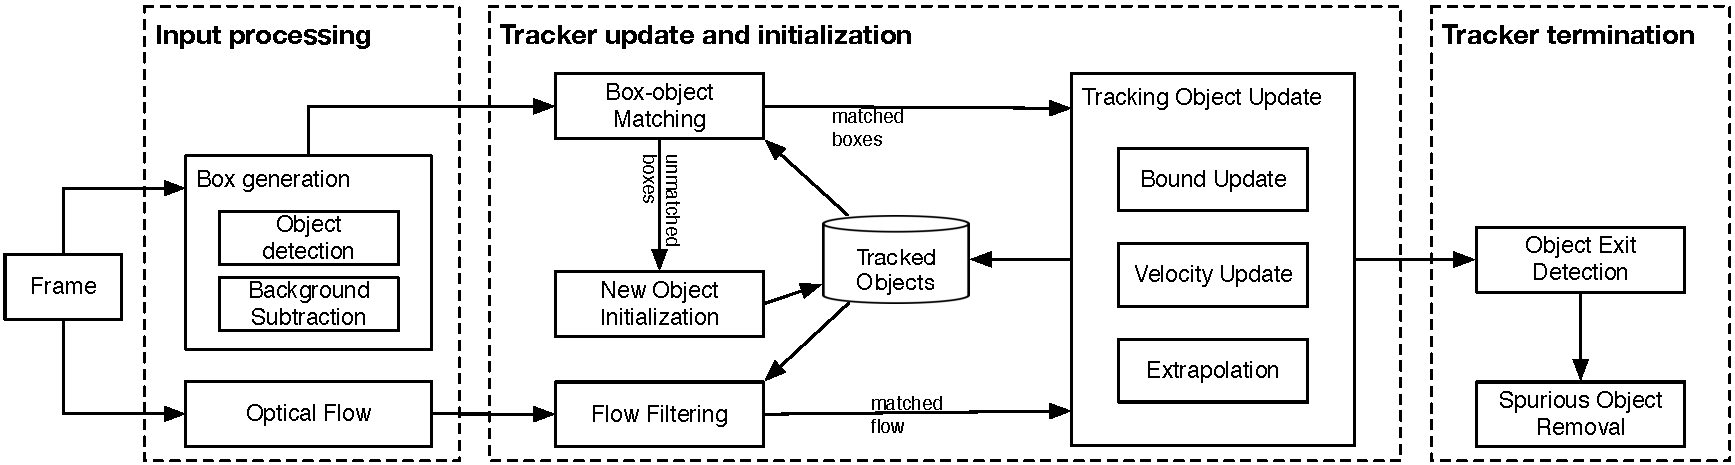
\includegraphics[width=\linewidth]{./img/kalmanFilterTracker.pdf}
\end{center}
    % \vspace{-1em}
   \caption{Overview of proposed system. Separate Kalman filter state is initialized, maintained and terminated for each tracked object. The state is updated based on matching input from background subtraction, object detection and optical flow.}
\label{fig:kf-tracker-workflow}
% \vspace{-1em}
\end{figure}
%We propose an efficient framework based on Kalman Filter, which is jointly updated by background subtraction model, detector and optical flow.
\ref{fig:kf-tracker-workflow} describes the workflow of our automatic tracking application. We first apply background subtraction and object detector on each frame. This generates two sets of candidate boxes, which are used to initialize and update trackers. Each tracker is represented by an individual Kalman filter \cite{grewal2011kalman}. 
Optical flow is also computed. Any flow that matches a tracked object both by location and velocity, is used for tracker update. Tracking is terminated based on object location, velocity and time; short-lived or otherwise spurious objects are filtered out.

\subsection{Model definition}

% \subsection{Kalman filtering for fusing multiple inputs} \label{section:kalmanFilter}

% Given the pros and cons of above methods, we aim to combine them into a single system where the strengths of one method may compensate for the shortcomings of another. For this, we use Kalman filtering, both for its suitability in combining the results of these different methods, and for its ability to compute a smooth estimate from noisy input \cite{grewal2011kalman}. 
% %Kalman filter \cite{grewal2011kalman} is a recursive state estimator of linear dynamic system, with numerous applications in time series analysis, such as navigation, robotic control and signal processing. 

We use Kalman filter to smooth out the noises in the observed measurements by the aforementioned components and more importantly, to integrate the strengths and compensate the weakness of each component. The \emph{prediction} by its linear model is \emph{corrected} with measurements observed over time, therefore the generated estimation is much smoother despite the noises in measurement input. 
%combine the aforementioned unstable components, both for its suitability in combining multiple potentially conflicting measurements into a single coherent model, and for its ability to compute a smooth estimate from noisy input. 
To model the state change, a discrete-time controlled process is modeled as linear stochastic difference equation \cite{Welch:1995:IKF:897831}, state at time $k$ is a linear combination of its previous state $\mathbf{x_{t-1}}$ at time $t-1$
% , a control signal $\mathbf{u}_{k-1}$ 
and the process noise $\mathbf{w}_{t-1}$:
% \setlength{\abovedisplayshortskip}{0pt}
% \setlength{\belowdisplayshortskip}{0pt}
\begin{equation}
  % \mathbf{x}_k = A\mathbf{x}_{k-1} + B\mathbf{u}_{k-1}+\mathbf{w}_{k-1},  
  \mathbf{x}_k = A\mathbf{x}_{t-1} + \mathbf{w}_{t-1}, \label{eq:kf-transition}
\end{equation}
where $A$ is the state transition model.
% , $B$ is a control-input model applied on control vector $\mathbf{u_{k-1}}$. 
In our case, A models how object move on the frame along time, presumably satisfies constant acceleration movement.
There is also measurement $\mathbf{z}\in \mathbb{R}^{m}$ formulated as
\begin{equation}
\mathbf{z}_t = H\mathbf{x}_t+\mathbf{v}_t.
\label{eq:kf-measurement}
\end{equation}
Here $H$ is the measure model, which observation to correct prediction from previous step. $\mathbf{w}_t$ in \ref{eq:kf-transition} and $\mathbf{v}_t$ in \ref{eq:kf-measurement} are process and measurement noise respectively. They are assumed independent of each other and zero-mean Gaussian, with $Q$ and $R$ as process noise covariance and measurement noise covariance, respectively.
\begin{align}
\begin{split}
p(\mathbf{w})\sim \mathcal{N}(0, Q)\\
p(\mathbf{v})\sim \mathcal{N}(0, R)
\end{split}
\end{align}
The recursive process of Kalman filter contains two steps: time update (prediction) and measurement update (correction). Both steps are applied at time $k$, indicated by subscripts below.
For such a continuous system, we define a time unit $dt$, which is the time interval we perform an update, in our case, the time between two consecutive frames. Each variable has its own value at a certain time step $t$, indicated by the subscript. The prediction is performed as follows: 
% \setlength{\abovedisplayskip}{2pt}
% \setlength{\belowdisplayskip}{2pt}
% \noindent\textbf{Prediction:}
\begin{align}
\begin{split}
\mathbf{\hat{x}}^{\mhyphen}_t & = A\mathbf{\hat{x}}_{t-1}\\
P^\mhyphen_t & = AP_{t-1}A^T + Q 
\end{split}
\label{eq:kf-predict}
\end{align}

Here $\mathbf{\hat{x}}_{t-1}$ and $\mathbf{\hat{x}}^{\mhyphen}_t$ are internal states before and after prediction at time $t$. $P_{t-1}$ and $P^\mhyphen_t$ are prior and post error covariances, and $Q$ is the process noise covariance. In our case, we define 
% Here $A$ is the linear transition model to describe the state change over time.
% Each tracked object has a Kalman filter and we have 
the internal state a 10-dimensional vector: $$\mathbf{x}=[x, y, w, h, x', y', w', h', x'', y''],$$ corresponding to the object's top left location $(x, y)$, size $(w, h)$, as well as the velocity ($x',y'$), rate of growth ($w',h'$) and acceleration $(x'', y''$), respectively.
The dynamic model $A$ is defined based on the physics equation of displacement with velocity and acceleration. With the assumption that the object has constant acceleration within $dt$, we have:
% \setlength{\abovedisplayskip}{2pt}
% \setlength{\belowdisplayskip}{2pt}
\begin{align}
\begin{split}
  x_t & = x_{t-1} + x'_{t-1}\cdot dt+\tfrac{1}{2}\cdot x''_{t-1}\cdot dt^2\\
  y_t & = y_{t-1} + y'_{t-1}\cdot dt+\tfrac{1}{2}\cdot y''_{t-1}\cdot dt^2\\
  x'_t & = x'_{t-1} + x''_{t-1}\cdot dt\\
  y'_t & = y'_{t-1} + y''_{t-1}\cdot dt.
\end{split}
\label{eq:motion-model-r}
\end{align}

For width and height, we instead assume constant growth rate within $dt$, thus
\begin{align}
\begin{split}
  w_t & = w_{t-1} + w'_{t-1}\cdot dt\\
  h_t & = h_{t-1} + h'_{t-1}\cdot dt
\end{split}
\label{eq:motion-model-v}
\end{align} 

% . In our case, we use a constant acceleration movement model; $B$ is a control-input model, but not used here. $H$ is a measurement model, mapping measurements to the states in $\mathbf{\hat x}$. Finally, $Q$ and $R$ are process noise covariance and measurement noise covariance, respectively.

% Thus, $A$ and $Q$ describe feasible object movements, $H$ can accommodate any number of measurements, and $R$ incorporates the expected error in each measurement, as well as correlations between measurements. Below, we describe our proposed system, consisting of central per-object Kalman filter, with detection, background subtraction and optical flow as input. 

% In the prediction step, preliminary prediction of state $\mathbf{\hat{x}^{\mhyphen}}$ and process noise covariance $P^\mhyphen_k$ is made based on value at previous time step. In measurement update step, Kalman gain $K_k$ is first computed and used to correct state estimation $\mathbf{\hat{x}_k}$ and process noise covariance $P_k$. Note that the Kalman gain $K_k$ indicates how much the measurement $\mathbf{z_k}$ is trusted to update the estimation ((\ref{eq:correct})). We update our model with different measurements confidence, by manipulating the measurement noise covariance $R$, in order to have desirable $K_k$. See \cite{Welch:1995:IKF:897831} for more details about Kalman filtering.

% \textbf{Correction:}
After prediction, the estimated state $\mathbf{\hat{x}^{\mhyphen}_t}$ is corrected by an observed measurement $\mathbf{z}$ at each time step by the steps below: 
\begin{align}
\begin{split}
K_t & = P^{\mhyphen}_t H^T(HP^{\mhyphen}_t H^T+R)^{-1}\\
\mathbf{\hat{x}_t} & = \mathbf{\hat{x}^{\mhyphen}_t} + K_t(\mathbf{z_t} - H\mathbf{\hat{x}^{\mhyphen}_t)}\\
P_t & = (I-K_tH)P^{\mhyphen}_t
\end{split}
\label{eq:kf-correct}
\end{align}

In our case, we have a 10-dimensional measurement vector: 
$$\mathbf{z}=[x^{bg}, y^{bg}, w^{bg}, h^{bg}, x^{det}, y^{det}, w^{det}, h^{det}, v_x, v_y],$$ 
which represents the top left coordinates $(x, y)$, width $(w)$, height $(h)$, reported by background subtraction $bg$ and detector $det$, separately, as well as the velocity $(v_x, v_y)$ reported by optical flow estimation. 
The measurement model $H$ is a 10-by-10 matrix of zeros except for ones at $(0, 0),$ $(1, 1),$ $(2, 2),$ $(3, 3),$ $(0, 4),$ $(1, 5),$ $(2, 6),$ $(3, 7),$ $(4, 8),$ $(5,9)$, signifying that the background and detector boxes directly measure $x$, $y$, $w$, and $h$, and that optical flow directly measures $x'$ and $y'$. In other words, there are no direct measurements of $w'$, $h'$, $x''$ or $y''$ since they are not observable.
$R$ is the measurement noise covariance, indicating the noisiness of measurement. By manipulating the measurement noise covariance $R$, we compute a Kalman gain $K_t$, indicating the weight of the measurement to update the corresponding prediction. 
%Finally, $Q$ and $R$ are set based on the observed statistics of each variable (based on our ground truth data). 


\subsection{Measurement acquisition}

%We define the object location $(x, y)$, size $(w, h)$ and velocity $(u, v)$ as our measurement to update the internal states. 
%This section below describes how we generate less noisy measurement values from fallible background subtraction model, detector and optical flow.
None of our input measurements: background subtraction, object detection and optical flow, correspond directly to a single tracked object. Instead, they generate boxes and flow indications for an entire frame.
To produce input to an individual tracked object's filter, we first compute a matching of input data to tracked objects, then apply the matched boxes and flow to the corresponding object's Kalman filter state. 

\textbf{Background subtraction and object detection:}
Both background subtraction and object detection generate bounding boxes $\{x,y,w,h\}$. We only take those consistent with tracker's current state as the measurement. For each Kalman filter, the best matching box as measurement maximizes the total overlap between the predicted bounds of internal filter, and the bounds of the measured boxes. Boxes must overlap with the predicted state in order to be considered a match. Any remaining boxes are used to initialize new tracked objects. 

\textbf{Optical flow:}  
%Figure \ref{fig:flowFilter} shows the process of optical flow filtering.
Optical flow reports velocity on a pixel-by-pixel basis, with many erroneous flow vectors due to the aperture and turbulence problems described earlier. To produce a velocity measurement from the optical flow field for a single object, we first denoise the flow field by forward-backward error thresholding, as described in \cite{kalal2010forward}. We then filter the flow by location, velocity magnitude and direction. In particular, we only consider flow vectors that originate from the location of the object in the previous frame, follow the similar direction (within in $45^\circ$) of the previous state -- to reduce the effect of turbulence problem, and only keep those vectors that fall within twice the error covariance 
(available in $P$, diagonal entries corresponding to the object velocity in $\mathbf{\hat x}$), using the simplifying assumption that flow errors follow a normal distribution. 
%
%Note that these operations are efficiently done on frame level and shared among all objects. When flow vectors are used to compute displacement of single object, we make use of the internal states to help flow filtering. The internal state $(v^x, v^y)$ is the direction of the object computed accumulatively over previous time steps, which indicates the rough direction of the flow. We discard flows that differ with internal state $(v^x, v^y)$ in direction and magnitude, which is especially useful when occlusion happens.
Finally we use the mean of the remaining flow vectors on horizontal and vertical direction, respectively, as the optical flow measurement for the object. 

%% \begin{figure}[!htbp]
%% \begin{center}
%%  \includegraphics[width=\linewidth]{./img/flowFiltering.pdf}
%% \end{center}
%%    \caption{Optical flow filtering.}
%% \label{fig:flowFilter}
%% \end{figure}
\subsection{Model update}

The measurements above are directly plugged into \ref{eq:kf-correct}, however, are of different quality, and oftentimes some of the measurements are missing entirely. For example, the invalid foreground is generated when occlusion happens; detector misses a small-sized object, or aperture problem gives zero movement of object.
We address these problems by varying the measurement noise covariance accordingly, which in turn causes the Kalman filter to choose a gain $K$ that maximizes the quality of the internal state. Recall in \ref{eq:kf-correct}, a large measurement covariance $Q$ would result in a smaller $K$, therefore the measurement weights less in correction. When a measurement is missing, we use the value already in $\mathbf{\hat x}$ as a proxy, and set the covariance to $\infty$. Consequently, once none of the three measurements is available, the tracker merely relies on the internal prediction, which we call \emph{extrapolation}. The tracker could still generate tracking results by the internal linear model during extrapolation. The other two cases in \ref{fig:kf-tracker-workflow} are when at least one bounding box is available (bound update) or only optical flow is obtained (velocity update).

We also apply error gating to the background subtraction and object detection measurements. %We assign measurements different weights for update by manipulating the measurement covariance. 
For example, foreground bounding box that is well overlapped with tracked objects (more than $30\%$ overlap) has a higher confidence than those with other bounding boxes around. Similarly, optical flow have a lower confidence with zero value on both directions, since we have no idea whether the object is still or the aperture problem happens.
%A matched measurement box that has insufficient overlap (below 30\%) with the tracker state is treated as missing. 
In addition, as described in \S\ref{sec:tracker-preliminary}, the three measurement types naturally have different error covariances. Although detector has a higher missing rate, the recall is also high. Therefore, measurement from detector has a smaller noise covariance value than those from background model.

%We propose three different kinds of update mechanisms: bound update, flow update and extrapolation, as shown in Figure \ref{fig:workflow}.
%Bound update is only used when the box is of high confidence, usually applied to moving objects without any occlusion; flow update is when we are not sure about the box, but we have relatively confident optical flow vector, this happens when occlusion or background crashes with illumination change. When neither box nor optical flow is reliable, we hold the state and only predict without correction, this is called extrapolation. Common case is that tracked object is partially occluded or noise. Each update is executed with different measurement covariance based on the certainty of the box and flow vector. 
%Recall that in section \ref{section:kalmanFilter} we mentioned that by tuning measurement covariance $R$, we are able to change the weight (Kalman gain $K_k$ in (\ref{eq:predict_gain})) of measurement in correction step. More specifically, when we update with both bounds and optical flow vector, we make measurement covariance $Q$ small for the location $(x, y, w, h)$ and velocity $(u, v)$, resulting a large $K_k$; if we use flow update, only entries of $Q$ corresponding to velocity $(u, v)$ are given a small value. When in extrapolation mode, measurement covariance matrix will be set a high value, indicating the measurements for neither location nor velocity are certain.
% \begin{table}[!htbp]
% \footnotesize
% \centering
% \caption{Kalman filter update schemes.}
% \begin{tabular}{|m{0.16\linewidth}|m{0.22\linewidth}|m{0.22\linewidth}|m{0.2\linewidth}|}
%   \hline
%       ~   & \textbf{Update condition} & \textbf{Operation}& \textbf{Example case}  \\ \hline  
%   Bound update    &   High confidence in both box and velocity.   & Small $Q$ value for $(x, y, w, h , u, v)$. & Single object without occlusion.\\ \hline
%   Flow update         & Low confidence in box, high confidence in velocity. &  Large $Q$ value for $(x, y, w, h)$, small value for $(u, v)$. & Background model failure or miss detection.\\ \hline
%   Extrapolation       & Low confidence in both box and velocity. &  Large $Q$ value for $(x, y, w, h , u, v)$. & Occlusion or noise.\\ \hline
% \end{tabular}
% \label{table:udpate}
% \end{table}